\documentclass{eptcs}
\providecommand{\event}{\GAM 2015}
%\documentclass{llncs}
%\usepackage{lncs}

\usepackage{amsmath,latexsym,amsfonts,amssymb,amsthm,verbatim}
\usepackage{rotating,graphs,stmaryrd}
\usepackage{subfig,pgf,xcolor,tikz}
\usepackage{cite}
\usepackage{breakurl}

% ENVIRONMENTS --------------------------

%\theoremstyle{remark}
\newtheorem{example}{Example}


% MISC ----------------------------------

\newcommand{\red}[1]{\textcolor{red}{#1}}
\newcommand{\blue}[1]{\textcolor{blue}{#1}}
\newcommand{\ttt}{\texttt}
\newcommand{\csp}{\hspace{.2em}}


% FORMULAS ------------------------------------

\newcommand{\mylabel}[1]{ \left\{
 \begin{array}{@{}l@{}} #1 \end{array} \right\}
}

\newcommand{\lvar}[1]{\mathtt{#1}}

\newcommand{\Z}{\mathbb{Z}}
\newcommand{\N}{\mathbb{N}}

\newcommand{\mtt}{\mathtt}
\newcommand{\mrm}{\mathrm}
\newcommand{\msf}{\mathsf}

\newcommand{\C}{\mathrm{Char}}
\newcommand{\Adr}{\mathrm{Adr}}
\newcommand{\Prog}{\mathrm{P}}

\newcommand{\fail}{\mathrm{fail}}
\newcommand{\g}{\mathrm{gra}}
\newcommand{\reg}{\mathrm{reg}}
\newcommand{\s}{\mathrm{s}}

\newcommand{\R}{\mathcal{R}}
\renewcommand{\L}{\mathcal{L}}
\newcommand{\I}{\mathcal{I}}
\newcommand{\G}{\mathcal{G}}
\newcommand{\A}{\mathcal{A}}
\renewcommand{\S}{\mathcal{S}}

\newcommand{\sos}{\mathrm{sos}}
\newcommand{\Sem}[1]{\llbracket{#1}\rrbracket}
\newcommand{\trans}[1]{\tau\llbracket{#1}\rrbracket}
\newcommand{\Gbot}{\mathcal{G}_{\bot}}

\newcommand{\X}{\mathrm{X}}
\newcommand{\V}{\mathrm{V}}
\newcommand{\E}{\mathrm{E}}
\newcommand{\D}{\mathrm{D}}
\newcommand{\tuple}[1]{\langle#1\rangle}
\newcommand{\la}{\langle}
\newcommand{\ra}{\rangle}
\newcommand{\dom}{\mathrm{Dom}}

\newcommand{\x}{\mathtt{x}}
\newcommand{\y}{\mathtt{y}}
\newcommand{\z}{\mathtt{z}}

\newcommand{\ifte}[3]{\mathtt{if}\ #1\ \mathtt{then}\ #2\ \mathtt{else}\ #3}
\newcommand{\ift}[2]{\mathtt{if}\ #1\ \mathtt{then}\ #2}
\newcommand{\tryt}[2]{\mathtt{try}\ #1\ \mathtt{then}\ #2}
\newcommand{\tryte}[3]{\mathtt{try}\ #1\ \mathtt{then}\ #2\ \mathtt{else}\ #3}
\newcommand{\noteq}{\mathrel{\text{\texttt{!=}}}}

\renewcommand{\bar}[1]{\overline{#1}}
\newcommand{\wt}[1]{\widetilde{#1}}
\newcommand{\wh}[1]{\widehat{#1}}

\newcommand{\ul}[1]{\underline{#1}}


% REWRITE RELATIONS ---------------------------

% Abstract reduction and term rewriting -------

\newcommand{\symto}{\leftrightarrow}

\newcommand{\DSto}{\mathop{\to}\limits}
\newcommand{\DSsymto}{\mathop{\symto}\limits}

\newcommand{\symredu}{\Leftrightarrow_{\R}}

\newcommand{\dder}{\Rightarrow}
\newcommand{\ldder}{\Leftarrow}
\newcommand{\der}{\Rightarrow^*}
\newcommand{\lder}{\Leftarrow^*}

\newcommand{\DSdder}{\mathop{\Rightarrow}\limits}
\newcommand{\DSldder}{\mathop{\Leftarrow}\limits}
\newcommand{\DSder}{\DSdder^*}
\newcommand{\DSlder}{\DSldder^*}

\newcommand{\DSlongdder}{\mathop{\Longrightarrow}\limits}
\newcommand{\DSllongdder}{\mathop{\Longleftarrow}\limits}


% GRAPHS -------------------------------------

\newcommand{\bluenodecolour}{\graphnodecolour(0,.6,1)}
\newcommand{\rednodecolour}{\graphnodecolour(1,.03,.03)}
\newcommand{\greennodecolour}{\graphnodecolour(0,1,0)}
\newcommand{\grey}{\graphnodecolour{.75}}
\newcommand{\dashed}{\graphlinedash{4 2}}

\newcommand{\script}{\scriptsize}
\newcommand{\fs}{\footnotesize}
\newcommand{\op}[3]{\textnode{#1}(#2){$\mathtt{#3}$}[\graphlinecolour{1}]}
\newcommand{\smallnode}{\graphnodesize{0.30}}
\newcommand{\nodegraph}[1]{% 
 \graphlinewidth{.01}
 \graphlinecolour{0}
 \graphnodecolour{1}
 \graphnodesize{.4}
 \begin{graph}(.4,.2)
  \roundnode{n}(.2,.1)\autonodetext{n}{#1}
 \end{graph}
}
\newcommand{\edgegraph}{% 
 \graphlinewidth{.01}
 \graphlinecolour{0}
 \graphnodecolour{1}
 \graphnodesize{.2}
 \grapharrowlength{.15}
 \grapharrowwidth{.45}
 \begin{graph}(1,.2)
  \roundnode{s}(.2,.1)\autonodetext{s}[s]{\tiny $s$}
  \roundnode{t}(.8,.1)\autonodetext{t}[s]{\tiny $t$}
  \diredge{s}{t}
 \end{graph}
}
\newcommand{\parrule}{% 
 \graphlinewidth{.01}
 \graphlinecolour{0}
 \graphnodecolour{1}
 \graphnodesize{.2}
 \grapharrowlength{.15}
 \grapharrowwidth{.45}
 \begin{graph}(.8,.2)
  \freetext(.6,0){par:}
 \end{graph}
 \begin{graph}(1,.2)
  \roundnode{s}(.2,.1)\autonodetext{s}[s]{\tiny 1}
  \roundnode{t}(.8,.1)\autonodetext{t}[s]{\tiny 2}
  \dirbow{s}{t}{.1}
  \dirbow{s}{t}{-.1}
 \end{graph}
 \begin{graph}(.4,.2)
  \freetext(.2,.1){\small $\dder$}
 \end{graph}
 \begin{graph}(1,.2)
  \roundnode{s}(.2,.1)\autonodetext{s}[s]{\tiny 1}
  \roundnode{t}(.8,.1)\autonodetext{t}[s]{\tiny 2}
  \diredge{s}{t}
 \end{graph}
}
\newcommand{\seqrule}{% 
 \graphlinewidth{.01}
 \graphlinecolour{0}
 \graphnodecolour{1}
 \graphnodesize{.2}
 \grapharrowlength{.15}
 \grapharrowwidth{.45}
 \begin{graph}(.8,.2)
  \freetext(.6,0){seq:}
 \end{graph}
 \begin{graph}(1.6,.2)
  \roundnode{s}(.2,.1)\autonodetext{s}[s]{\tiny 1}
  \roundnode{d}(.8,.1)
  \roundnode{t}(1.4,.1)\autonodetext{t}[s]{\tiny 2}
  \diredge{s}{d}
  \diredge{d}{t}
 \end{graph}
 \begin{graph}(.4,.2)
  \freetext(.2,.1){\small $\dder$}
 \end{graph}
 \begin{graph}(1,.2)
  \roundnode{s}(.2,.1)\autonodetext{s}[s]{\tiny 1}
  \roundnode{t}(.8,.1)\autonodetext{t}[s]{\tiny 2}
  \diredge{s}{t}
 \end{graph}
}


\usetikzlibrary{arrows,fit,backgrounds}
\tikzset{arrowin/.style={<-,>=latex,semithick},arrowout/.style={->,>=latex,semithick},root/.style={circle,draw,line width=2pt},box/.style={rectangle, rounded corners, minimum width=1cm, minimum height=1cm,text centered, draw=black}}


\begin{document}

\title{A Reference Interpreter for the Graph Programming Language GP 2}

\author{Christopher Bak, Glyn Faulkner, Detlef Plump and Colin Runciman
    \institute{Department of Computer Science\\
               The University of York, UK}
}

\def\authorrunning{C. Bak, G. Faulkner, D. Plump \& C. Runciman} 
\def\titlerunning{A Reference Interpreter for GP2}

\maketitle
\thispagestyle{empty}


\begin{abstract}
GP 2 is an experimental programming language
for computing by graph transformation.
An initial interpreter for GP 2, written
in the functional language Haskell, provides
a concise and simply structured reference
implementation.
Despite its simplicity, the performance of
the interpreter is sufficient for the
comparative investigation of a range of test
programs.
It also provides a platform for the development
of more sophisticated implementations.
\end{abstract}

\section{Introduction}

GP~2 is an experimental programming language in which the major part of
the computational state is a labelled directed graph, and the basic
units by which computational progress is made are subgraph-rewriting
rules.
Choices of rules and subgraphs are non-determinstic, and some of
the control structures above the level of rules involve back-tracking.

The implementation of such a programming language poses some
interesting challenges and opportunities.
Our ultimate goal is to produce a compiler from GP~2 to
high-performance executable code.
This paper reports a first stage towards that goal, the development
of a \emph{reference interpreter} for GP~2.
By this we mean an interpreter written with the main aim of
being clear, concise and correct.
Where there are design choices, simplicity of
definition takes priority over other considerations
such as performance and the richness of functionality.

Section~\ref{sec:graph-programs} outlines and illustrates the GP~2 language
graph-programming language.
Section~\ref{sec:benchmark} presents a small set of test programs
written in GP~2.
Section~\ref{sec:usesrequirements} considers the expected uses of
a reference interpreter, and consequent requirements.
Section~\ref{sec:implementation} describes our reference interpreter for
GP~2.
Section~\ref{sec:performanceevaluation} sets out the measured results of using the reference
interpreter to evaluate the test programs in Section~\ref{sec:benchmark}.
Section~\ref{sec:relatedandfuture} briefly discusses related work and
indicates some of our own expected lines of future work.
Section~\ref{sec:conclusions} draws overall conclusions from our work
on the reference interpreter for GP~2.


\section{Graph Programs}
\label{sec:graph-programs}

This paper focusses on GP~2, a successor to the graph programming language GP \cite{Plump09a,Plump12a}.
GP is a domain-specific language which aims to support formal reasoning on graph programs (see \cite{Poskitt-Plump12a} for a Hoare-logic approach to verifying GP programs). We give a brief introduction to GP~2, mainly by example. The definition of the language, including a formal operational semantics, can be found in \cite{Plump12a}. 

A graph program consists of declarations of conditional graph transformation rules and macros, and exactly one main command sequence. Graphs are directed and may contain  loops and parallel edges. The rules operate on a \emph{host graph}\/ (or input graph) whose nodes and edges may be labelled.

Labels are of type \texttt{int} (for integers), \texttt{char} (for characters), \texttt{string} (for character strings), \texttt{atom} or \texttt{list}, where \texttt{atom} is the union of \texttt{int}, \texttt{char} and \texttt{string}. Atoms are considered as lists of length one, hence integers and strings are also lists. Given lists $\mtt{x}$ and $\mtt{y}$, their concatenation is written \texttt{x:y} (not to be confused with the list-cons operator in Haskell). 
We proceed by discussing two example programs.

\begin{example}[Transitive Closure]
The principal programming constructs in GP~2 are conditional graph-transformation rules labelled with expressions. The program in Figure \ref{fig:transitive-closure} applies the single rule \ttt{link} \emph{as long possible} to a host graph. In general, any subprogram can be iterated by applying \ttt{!} as a postfix operator.

\begin{figure}[htb]
\begin{center}
 \input{Programs/trans_closure.prog}
\end{center}
%\vspace{-.5\baselineskip}
\caption{Program for transitive closure}\label{fig:transitive-closure}
\end{figure}

Applying \ttt{link} amounts to non-deterministically selecting a subgraph of the host graph that matches \ttt{link}'s left graph, and adding to it an edge from node 1 to node 3 provided there is no such edge (with any label). The application condition ensures that the program terminates and extends the host graph with a minimal number of edges.

A graph is \emph{transitive} if for each directed path from a node $v$ to another node $v'$, there is an edge from $v$ to $v'$.  Given any graph $G$, the program in Figure \ref{fig:transitive-closure} produces the smallest transitive graph that results from adding unlabelled edges to $G$.\footnote{``Unlabelled'' edges are actually labelled with the empty list.} This graph is unique up to isomorphism and requires at most $n^2$ applications of \ttt{link}, where $n$\/ is the number of nodes in $G$. \qed
\end{example}
  

\begin{example}[Vertex Colouring]
The program in Figure \ref{fig:vertex-colouring} assigns a \emph{colour}\/ to each node of the host graph, such that non-loop edges have differently coloured endpoints. Positive integers are used as colours because, in general, an unbounded number of colours is needed. The program replaces each node label $l$\/ with $l{:}i$, where $i$\/ is the node's colour. In addition, the rule \ttt{init} shades nodes to prevent repeated application to the same node.
% (Nodes can be graphically \emph{marked}\/ by drawing them shaded or in one of the colours red, green or blue.)

\begin{figure}[htb]
\begin{center}
 \input{Programs/vertex-colouring.prog}
\end{center}
%\vspace{-.5\baselineskip}
\caption{Program for vertex colouring}\label{fig:vertex-colouring}
\end{figure}

Rule \ttt{inc} is applied to the host graph as long as there are edges with identically coloured endpoints. It can can be shown that this terminates after at most $n^2$ rule applications, where $n$\/ is the number of nodes. In contrast to the previous example program, \emph{different graphs may result}\/ from this process. In particular, there is no guarantee that the number of colours produced is minimal. For instance, Figure \ref{fig:colour_results} shows two different colourings produced for the same host graph.
\qed
\end{example}

\begin{figure}[htb]
\begin{center}
 \input{Graphs/colour_results.graph}
\end{center}
%\vspace{-.5\baselineskip}
\caption{Different results from vertex colouring}\label{fig:colour_results}
\end{figure}

\vspace{.5\baselineskip}
\noindent
\emph{Other program constructs.}
A GP~2 command not used in the example programs is a rule set $\mtt{\{}r_1,\dots,r_n\mtt{\}}$. This command \emph{non-deterministically} applies any of the rules to the current host graph. The application \emph{fails}\/ if none of the left-hand graphs in the rules matches a subgraph. Matches must be injective and are only valid if they do not result in \emph{dangling edges}.

Another construct not yet discussed is the branching command \ttt{if} $C$ \ttt{then} $P$ \ttt{else} $Q$, where $C$, $P$ and $Q$ are arbitrary command sequences. This is executed on a host graph $G$ by first executing $C$ on a copy of $G$. If $C$ succeeds, $P$\/ is executed on the original graph $G$; otherwise, $Q$ is executed on $G$. The command \ttt{try} $C$ \ttt{then} $P$ \ttt{else} $Q$ has a similar effect, except that $P$\/ is executed on the graph resulting from $C$'s execution. 

\section{Benchmark Programs}
\label{sec:benchmark}
 
Besides the programs for transitive closure and vertex colouring, we select four more programs for benchmarking.


\subsection{Shortest distances}

\begin{tabular}{lp{10.5cm}}
\ul{Input:} & A graph $G$ with a unique grey node $s$. All edge labels are non-negative integers. \\
\ul{Output:} & The graph obtained from $G$ by marking grey each node reachable from $s$ and replacing its label $l$\/ with $l{:}d$, where $d$\/ is the shortest distance from $s$. (A distance is the sum of the edge labels of a directed path.)
\end{tabular}
  
\begin{center}
\input{Programs/distances.prog}
\end{center}

\ul{Notes}
\begin{enumerate}
\setlength{\itemsep}{-.5ex}
\item The output is unique up to isomorphism.
\item The input requirement can be relaxed by allowing negative edge labels but forbidding directed cycles with a negative distance.
\end{enumerate}


\subsection{Recognising acyclic graphs}
\label{sec:acyclic}

\begin{tabular}{lp{10.5cm}}
\ul{Input:} & Any graph $G$. \\
\ul{Output:} & Graph $G$ if it is acyclic, otherwise the program fails.
\end{tabular}
  
\begin{center}
\input{Programs/acyclic.prog}
\end{center}


\subsection{Rooted 2-colouring}

\begin{tabular}{lp{10.5cm}}
\ul{Input:} & A non-empty, single-rooted, connected graph $G$ with atomic labels. \\
\ul{Output:} & If $G$\/ is 2-colourable, then the output is obtained from $G$\/ by marking each node with either red or blue. The source and target of each non-loop edge have different colours.\\
& If $G$\/ is not 2-colourable, then the output is $G$.
\end{tabular}

\begin{center}
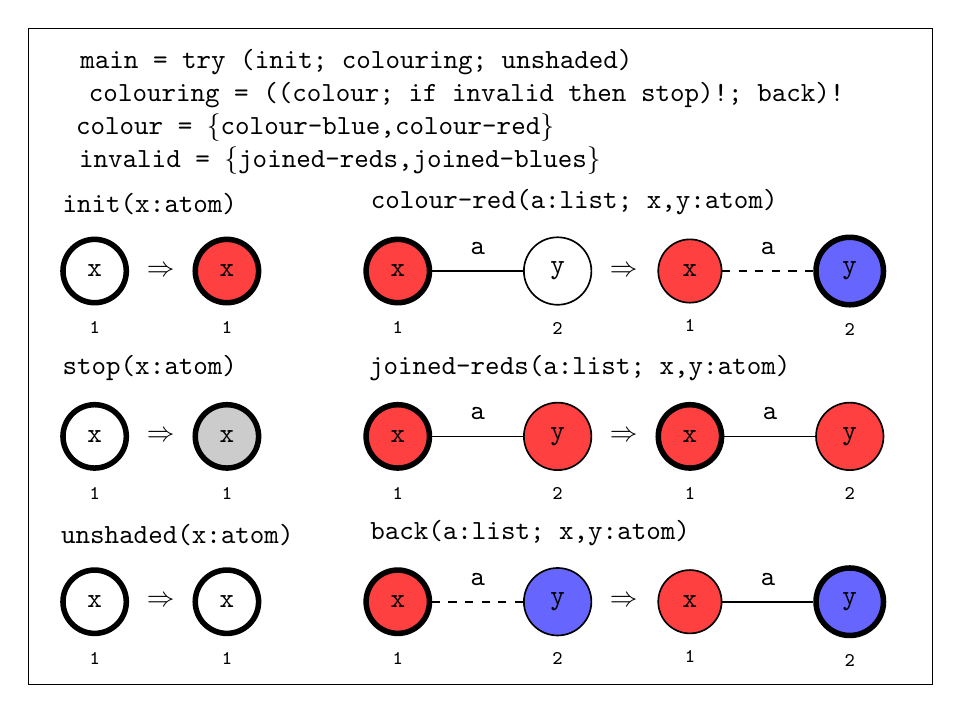
\begin{tikzpicture} [scale=0.7,align=center,auto,inner sep=2mm,arrowin,arrowout,font=\ttfamily]
\node at (4.75,3.8) {main = try (init; colouring; unshaded)};
\node at (6.75,3.2) {colouring = ((colour; if invalid then stop)!; back)!};
\node at (4,2.6) {colour = \{colour-blue,colour-red\}};
\node at (4.45,2) {invalid = \{joined-reds,joined-blues\}};

%init
\node at (0,0)[root,label=below:\scriptsize{1}]{x};
\node at (1.2,0){$\Rightarrow$};
\node at (1,0)[above=5mm] {init(x:atom)};
\node at (2.4,0)[root,fill=red!75,label=below:\scriptsize{1}]{x};

%stop
\begin{scope}[yshift=-3cm]
\node (l1) at (0,0)[root,label=below:\scriptsize{1}]{x};
\node at (1.2,0){$\Rightarrow$};
\node at (1,0)[above=5mm] {stop(x:atom)};
\node (r1) at (2.4,0)[root,fill=black!20,label=below:\scriptsize{1}]{x};
\end{scope}

%unshaded
\begin{scope}[yshift=-6cm]
\node (l1) at (0,0)[root,label=below:\scriptsize{1}]{x};
\node at (1.2,0){$\Rightarrow$};
\node at (1.5,0)[above=5mm] {unshaded(x:atom)};
\node (r1) at (2.4,0)[root,label=below:\scriptsize{1}]{x};
\end{scope}

%colour-red
\begin{scope}[xshift=5.5cm]
\node (l1) at (0,0)[root,fill=red!75,label=below:\scriptsize{1}]{x};
\node (l2) at (2.9,0)[inner sep = 2mm,circle,draw,label=below:\scriptsize{2}]{y}
   edge [-] node[above]{a} (l1);
\node at (4.1,0){$\Rightarrow$};
\node at (3.2,0)[above=5mm] {colour-red(a:list; x,y:atom)};
\node (r1) at (5.3,0)[circle,draw,fill=red!75,label=below:\scriptsize{1}]{x};
\node (r2) at (8.2,0)[root,fill=blue!60,label=below:\scriptsize{2}]{y}
  edge [-,dashed] node[above]{a} (r1);  
\end{scope}

%joined-reds
\begin{scope}[xshift=5.5cm,yshift=-3cm]
\node (l1) at (0,0)[root,fill=red!75,label=below:\scriptsize{1}]{x};
\node (l2) at (2.9,0)[circle,draw,fill=red!75,label=below:\scriptsize{2}]{y}
  edge [-] node[above]{a} (l1);
\node at (4.1,0){$\Rightarrow$};
\node at (3.3,0)[above=5mm] {joined-reds(a:list; x,y:atom)};
\node (r1) at (5.3,0)[root,fill=red!75,label=below:\scriptsize{1}]{x};
\node (r2) at (8.2,0)[circle,draw,fill=red!75,label=below:\scriptsize{2}]{y}
  edge [-] node[above]{a} (r1);
\end{scope}

%back
\begin{scope}[xshift=5.5cm,yshift=-6cm]
\node (l1) at (0,0)[root,fill=red!75,label=below:\scriptsize{1}]{x};
\node (l2) at (2.9,0)[circle,draw,fill=blue!60,label=below:\scriptsize{2}]{y}
  edge [-,dashed] node[above]{a} (l1);  
\node at (4.1,0){$\Rightarrow$};
\node at (2.4,0)[above=5mm] {back(a:list; x,y:atom)};
\node (r1) at (5.3,0)[circle,draw,fill=red!75,label=below:\scriptsize{1}]{x};
\node (r2) at (8.2,0)[root,fill=blue!60,label=below:\scriptsize{2}]{y}
  edge [-] node[above]{a} (r1);
\end{scope}

\draw (-1.2,4.4) rectangle (15.2,-7.5);

\end{tikzpicture}

\end{center}

\ul{Notes}
\begin{enumerate}
\setlength{\itemsep}{-.5ex}
\item The edges in the rules \ttt{colour}, \ttt{joined-reds} and \ttt{back} are \emph{bidirectional}. They matches host graph edges in either direction.
\end{enumerate}


\subsection{Generating Sierpinski triangles}

\begin{tabular}{lp{10.5cm}}
\ul{Input:} & A single node labelled with a non-negative integer $n$. \\
\ul{Output:} & The Sierpinski triangle of generation $n$.
\end{tabular}
  
\begin{center}
\input{Programs/sierpinski.prog}
\end{center}

\ul{Notes}
\begin{enumerate}
\setlength{\itemsep}{-.5ex}
\item The next page shows an example of a Sierpinski triangle.
\item The derivation length and the output size are exponential in $n$.
\end{enumerate}

\begin{figure}[htb]
 \begin{center}
  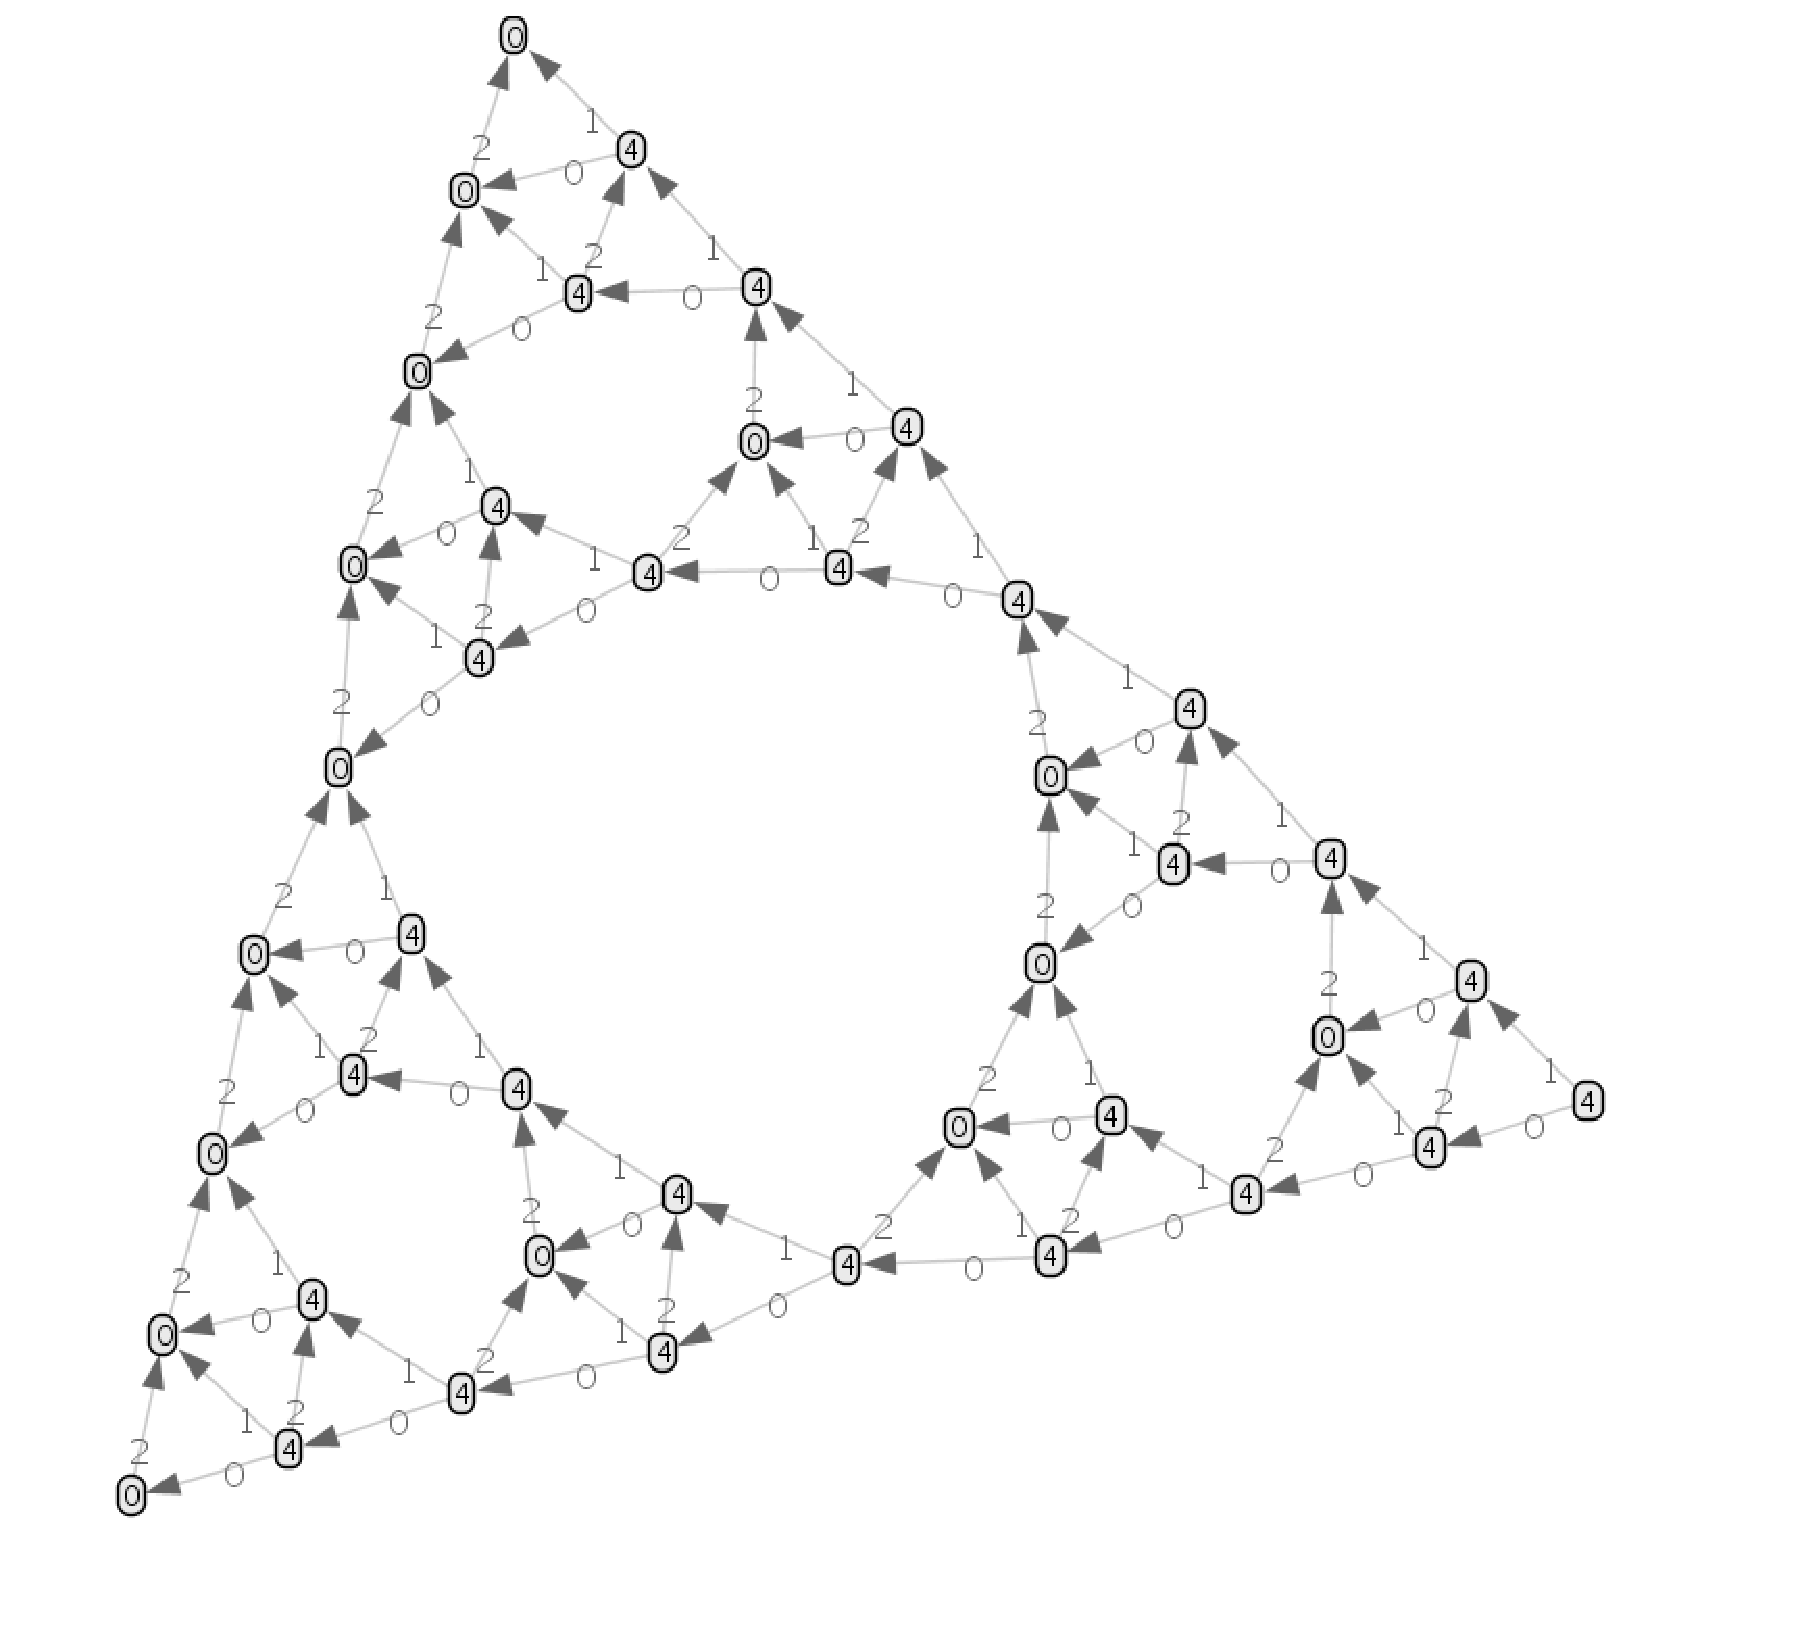
\includegraphics[scale=.4,angle=-15]{sierpinski-3.eps}
 \end{center}
\vspace*{-2.5cm}
\caption{Third generation Sierpinski triangle \label{fig:sierpinski}}
\end{figure}



\section{Reference Interpreters: Uses and Requirements}
\label{sec:usesrequirements}

A reference interpreter for a new programming language such as GP2
has several potential uses.
Each has consequences for the
way the reference interpreter is written and the
facilities it provides.

\vspace{.5\baselineskip}
\noindent
\emph{An arbiter for programmers.}
A programmer working in a new language needs to
know whether what they are writing is a valid
program, and whether the effect of executing it
is the effect they intend.
To resolve such issues, the programmer may want to
use a reference interpreter as a black box,
checking the output it produces given their
program as input.
Or they may wish to look at a salient part of the
source-code for the interpreter, to confirm some
aspect of the language they are unsure about.

It follows that a reference interpreter should
provide as output at least a report whether a
program is valid, and if so a clear representation
of the result when it is evaluated.
It also follows that the source-code for a
reference interpreter should
be organised in such a way that salient components
are easy to identify.
For ease of reading it should be written using a
consistent style in a modest subset of a suitable
high-level language.

\vspace{.5\baselineskip}
\noindent
\emph{An arbiter for implementors.}
An implementer of a programming language,
developing their own interpreter or compiler,
needs a standard against which to test the correctness
of their implementation.
There are two main respects in which any
implementation should agree with a reference interpreter
as a defining standard.
They should agree which programs are valid,
and for valid programs they should agree the results
of executing them.
Like application programmers, implementers too may
wish sometimes to use the reference interpreter as
a black box, but at other times to consult its
internal definitions. 

There are additional requirements for this use,
bearing in mind the likely development or generation
of many test programs.
The representation of the
reference interpreter's results for such programs
should be amenable to automated comparison.
This comparison presents particular challenges in GP~2 since
behaviour of programs may be non-deterministic,
or programs may not terminate, or both.
The number of test programs may be large
--- there may even be arbitrarily many test programs generated dynamically.
So although performance is not a design goal for the reference
interpreter, its performance should be good enough to
make such multi-test comparisons feasible.

\vspace{.5\baselineskip}
\noindent
\emph{A prototype for application developers.}
If no production compiler has been developed for the language,
or none is yet available to an application developer,
they may need to use a reference interpreter as
an initial development platform.

During the development of application programs, errors
are common.
So, for this use, a reference interpreter should provide
not only a check for valid programs, but a rapid check
with informative reports of errors.
Yet elaborate error handling must not obscure the
definitional style in which the interpreter is written.
Similarly, it is desirable to have the option of some
kind of trace or other informative report to shed
light on failures or unexpected results when a program
is evaluated.
Here again, the machinery must not obsure the basic
definitions for evaluation, nor should it impose heavy
performance costs when performance of the interpreter
has already been sacrificed in favour of simplicity.

\vspace{.5\baselineskip}
\noindent
\emph{A prototype for implementation developers.}
As well as using a reference interpreter to verify correctness,
implementers may wish to use it as the starting point in the
development of another interpreter or a compiler.
The whole course of such a development might even be defined as
the successive replacement of interpreter components by
alternatives giving higher performance, or richer information,
at the cost of greater complexity.
The advantage of this approach is that as each replacement
is introduced it can be checked as a new component in an already
tried system.

This use of a reference interpreter requires a
modular design with simple and clearly defined interfaces
between components.
Concerns should be separated so far as possible, avoiding
dependencies that are not strictly necessary.
Options for development by successive replacement may be further
increased by choosing a host programming system for the reference
interpreter that has a well-developed foreign-language interface. 


\section{Graph Programs}
\label{sec:graph-programs}

This paper focusses on GP~2, a successor to the graph programming language GP \cite{Plump09a,Plump12a}.
GP is a domain-specific language which aims to support formal reasoning on graph programs (see \cite{Poskitt-Plump12a} for a Hoare-logic approach to verifying GP programs). We give a brief introduction to GP~2, mainly by example. The definition of the language, including a formal operational semantics, can be found in \cite{Plump12a}. 

A graph program consists of declarations of conditional graph transformation rules and macros, and exactly one main command sequence. Graphs are directed and may contain  loops and parallel edges. The rules operate on a \emph{host graph}\/ (or input graph) whose nodes and edges may be labelled.

Labels are of type \texttt{int} (for integers), \texttt{char} (for characters), \texttt{string} (for character strings), \texttt{atom} or \texttt{list}, where \texttt{atom} is the union of \texttt{int}, \texttt{char} and \texttt{string}. Atoms are considered as lists of length one, hence integers and strings are also lists. Given lists $\mtt{x}$ and $\mtt{y}$, their concatenation is written \texttt{x:y} (not to be confused with the list-cons operator in Haskell). 
We proceed by discussing two example programs.

\begin{example}[Transitive Closure]
The principal programming constructs in GP~2 are conditional graph-transformation rules labelled with expressions. The program in Figure \ref{fig:transitive-closure} applies the single rule \ttt{link} \emph{as long possible} to a host graph. In general, any subprogram can be iterated by applying \ttt{!} as a postfix operator.

\begin{figure}[htb]
\begin{center}
 \input{Programs/trans_closure.prog}
\end{center}
%\vspace{-.5\baselineskip}
\caption{Program for transitive closure}\label{fig:transitive-closure}
\end{figure}

Applying \ttt{link} amounts to non-deterministically selecting a subgraph of the host graph that matches \ttt{link}'s left graph, and adding to it an edge from node 1 to node 3 provided there is no such edge (with any label). The application condition ensures that the program terminates and extends the host graph with a minimal number of edges.

A graph is \emph{transitive} if for each directed path from a node $v$ to another node $v'$, there is an edge from $v$ to $v'$.  Given any graph $G$, the program in Figure \ref{fig:transitive-closure} produces the smallest transitive graph that results from adding unlabelled edges to $G$.\footnote{``Unlabelled'' edges are actually labelled with the empty list.} This graph is unique up to isomorphism and requires at most $n^2$ applications of \ttt{link}, where $n$\/ is the number of nodes in $G$. \qed
\end{example}
  

\begin{example}[Vertex Colouring]
The program in Figure \ref{fig:vertex-colouring} assigns a \emph{colour}\/ to each node of the host graph, such that non-loop edges have differently coloured endpoints. Positive integers are used as colours because, in general, an unbounded number of colours is needed. The program replaces each node label $l$\/ with $l{:}i$, where $i$\/ is the node's colour. In addition, the rule \ttt{init} shades nodes to prevent repeated application to the same node.
% (Nodes can be graphically \emph{marked}\/ by drawing them shaded or in one of the colours red, green or blue.)

\begin{figure}[htb]
\begin{center}
 \input{Programs/vertex-colouring.prog}
\end{center}
%\vspace{-.5\baselineskip}
\caption{Program for vertex colouring}\label{fig:vertex-colouring}
\end{figure}

Rule \ttt{inc} is applied to the host graph as long as there are edges with identically coloured endpoints. It can can be shown that this terminates after at most $n^2$ rule applications, where $n$\/ is the number of nodes. In contrast to the previous example program, \emph{different graphs may result}\/ from this process. In particular, there is no guarantee that the number of colours produced is minimal. For instance, Figure \ref{fig:colour_results} shows two different colourings produced for the same host graph.
\qed
\end{example}

\begin{figure}[htb]
\begin{center}
 \input{Graphs/colour_results.graph}
\end{center}
%\vspace{-.5\baselineskip}
\caption{Different results from vertex colouring}\label{fig:colour_results}
\end{figure}

\vspace{.5\baselineskip}
\noindent
\emph{Other program constructs.}
A GP~2 command not used in the example programs is a rule set $\mtt{\{}r_1,\dots,r_n\mtt{\}}$. This command \emph{non-deterministically} applies any of the rules to the current host graph. The application \emph{fails}\/ if none of the left-hand graphs in the rules matches a subgraph. Matches must be injective and are only valid if they do not result in \emph{dangling edges}.

Another construct not yet discussed is the branching command \ttt{if} $C$ \ttt{then} $P$ \ttt{else} $Q$, where $C$, $P$ and $Q$ are arbitrary command sequences. This is executed on a host graph $G$ by first executing $C$ on a copy of $G$. If $C$ succeeds, $P$\/ is executed on the original graph $G$; otherwise, $Q$ is executed on $G$. The command \ttt{try} $C$ \ttt{then} $P$ \ttt{else} $Q$ has a similar effect, except that $P$\/ is executed on the graph resulting from $C$'s execution. 

\section{Benchmark Programs}
\label{sec:benchmark}
 
Besides the programs for transitive closure and vertex colouring, we select four more programs for benchmarking.


\subsection{Shortest distances}

\begin{tabular}{lp{10.5cm}}
\ul{Input:} & A graph $G$ with a unique grey node $s$. All edge labels are non-negative integers. \\
\ul{Output:} & The graph obtained from $G$ by marking grey each node reachable from $s$ and replacing its label $l$\/ with $l{:}d$, where $d$\/ is the shortest distance from $s$. (A distance is the sum of the edge labels of a directed path.)
\end{tabular}
  
\begin{center}
\input{Programs/distances.prog}
\end{center}

\ul{Notes}
\begin{enumerate}
\setlength{\itemsep}{-.5ex}
\item The output is unique up to isomorphism.
\item The input requirement can be relaxed by allowing negative edge labels but forbidding directed cycles with a negative distance.
\end{enumerate}


\subsection{Recognising acyclic graphs}
\label{sec:acyclic}

\begin{tabular}{lp{10.5cm}}
\ul{Input:} & Any graph $G$. \\
\ul{Output:} & Graph $G$ if it is acyclic, otherwise the program fails.
\end{tabular}
  
\begin{center}
\input{Programs/acyclic.prog}
\end{center}


\subsection{Rooted 2-colouring}

\begin{tabular}{lp{10.5cm}}
\ul{Input:} & A non-empty, single-rooted, connected graph $G$ with atomic labels. \\
\ul{Output:} & If $G$\/ is 2-colourable, then the output is obtained from $G$\/ by marking each node with either red or blue. The source and target of each non-loop edge have different colours.\\
& If $G$\/ is not 2-colourable, then the output is $G$.
\end{tabular}

\begin{center}
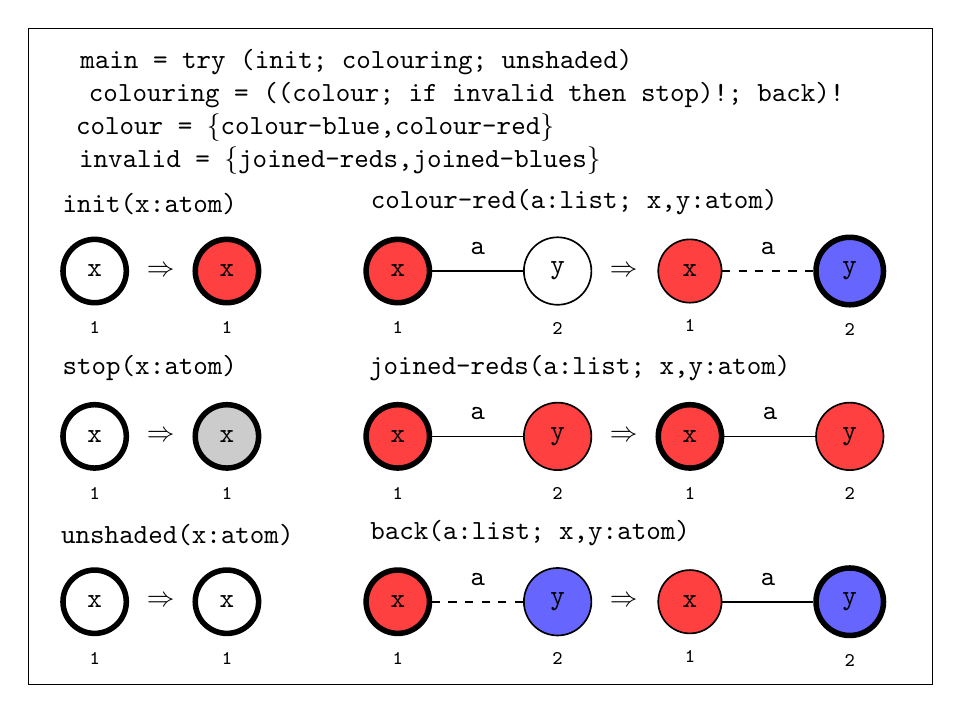
\begin{tikzpicture} [scale=0.7,align=center,auto,inner sep=2mm,arrowin,arrowout,font=\ttfamily]
\node at (4.75,3.8) {main = try (init; colouring; unshaded)};
\node at (6.75,3.2) {colouring = ((colour; if invalid then stop)!; back)!};
\node at (4,2.6) {colour = \{colour-blue,colour-red\}};
\node at (4.45,2) {invalid = \{joined-reds,joined-blues\}};

%init
\node at (0,0)[root,label=below:\scriptsize{1}]{x};
\node at (1.2,0){$\Rightarrow$};
\node at (1,0)[above=5mm] {init(x:atom)};
\node at (2.4,0)[root,fill=red!75,label=below:\scriptsize{1}]{x};

%stop
\begin{scope}[yshift=-3cm]
\node (l1) at (0,0)[root,label=below:\scriptsize{1}]{x};
\node at (1.2,0){$\Rightarrow$};
\node at (1,0)[above=5mm] {stop(x:atom)};
\node (r1) at (2.4,0)[root,fill=black!20,label=below:\scriptsize{1}]{x};
\end{scope}

%unshaded
\begin{scope}[yshift=-6cm]
\node (l1) at (0,0)[root,label=below:\scriptsize{1}]{x};
\node at (1.2,0){$\Rightarrow$};
\node at (1.5,0)[above=5mm] {unshaded(x:atom)};
\node (r1) at (2.4,0)[root,label=below:\scriptsize{1}]{x};
\end{scope}

%colour-red
\begin{scope}[xshift=5.5cm]
\node (l1) at (0,0)[root,fill=red!75,label=below:\scriptsize{1}]{x};
\node (l2) at (2.9,0)[inner sep = 2mm,circle,draw,label=below:\scriptsize{2}]{y}
   edge [-] node[above]{a} (l1);
\node at (4.1,0){$\Rightarrow$};
\node at (3.2,0)[above=5mm] {colour-red(a:list; x,y:atom)};
\node (r1) at (5.3,0)[circle,draw,fill=red!75,label=below:\scriptsize{1}]{x};
\node (r2) at (8.2,0)[root,fill=blue!60,label=below:\scriptsize{2}]{y}
  edge [-,dashed] node[above]{a} (r1);  
\end{scope}

%joined-reds
\begin{scope}[xshift=5.5cm,yshift=-3cm]
\node (l1) at (0,0)[root,fill=red!75,label=below:\scriptsize{1}]{x};
\node (l2) at (2.9,0)[circle,draw,fill=red!75,label=below:\scriptsize{2}]{y}
  edge [-] node[above]{a} (l1);
\node at (4.1,0){$\Rightarrow$};
\node at (3.3,0)[above=5mm] {joined-reds(a:list; x,y:atom)};
\node (r1) at (5.3,0)[root,fill=red!75,label=below:\scriptsize{1}]{x};
\node (r2) at (8.2,0)[circle,draw,fill=red!75,label=below:\scriptsize{2}]{y}
  edge [-] node[above]{a} (r1);
\end{scope}

%back
\begin{scope}[xshift=5.5cm,yshift=-6cm]
\node (l1) at (0,0)[root,fill=red!75,label=below:\scriptsize{1}]{x};
\node (l2) at (2.9,0)[circle,draw,fill=blue!60,label=below:\scriptsize{2}]{y}
  edge [-,dashed] node[above]{a} (l1);  
\node at (4.1,0){$\Rightarrow$};
\node at (2.4,0)[above=5mm] {back(a:list; x,y:atom)};
\node (r1) at (5.3,0)[circle,draw,fill=red!75,label=below:\scriptsize{1}]{x};
\node (r2) at (8.2,0)[root,fill=blue!60,label=below:\scriptsize{2}]{y}
  edge [-] node[above]{a} (r1);
\end{scope}

\draw (-1.2,4.4) rectangle (15.2,-7.5);

\end{tikzpicture}

\end{center}

\ul{Notes}
\begin{enumerate}
\setlength{\itemsep}{-.5ex}
\item The edges in the rules \ttt{colour}, \ttt{joined-reds} and \ttt{back} are \emph{bidirectional}. They matches host graph edges in either direction.
\end{enumerate}


\subsection{Generating Sierpinski triangles}

\begin{tabular}{lp{10.5cm}}
\ul{Input:} & A single node labelled with a non-negative integer $n$. \\
\ul{Output:} & The Sierpinski triangle of generation $n$.
\end{tabular}
  
\begin{center}
\input{Programs/sierpinski.prog}
\end{center}

\ul{Notes}
\begin{enumerate}
\setlength{\itemsep}{-.5ex}
\item The next page shows an example of a Sierpinski triangle.
\item The derivation length and the output size are exponential in $n$.
\end{enumerate}

\begin{figure}[htb]
 \begin{center}
  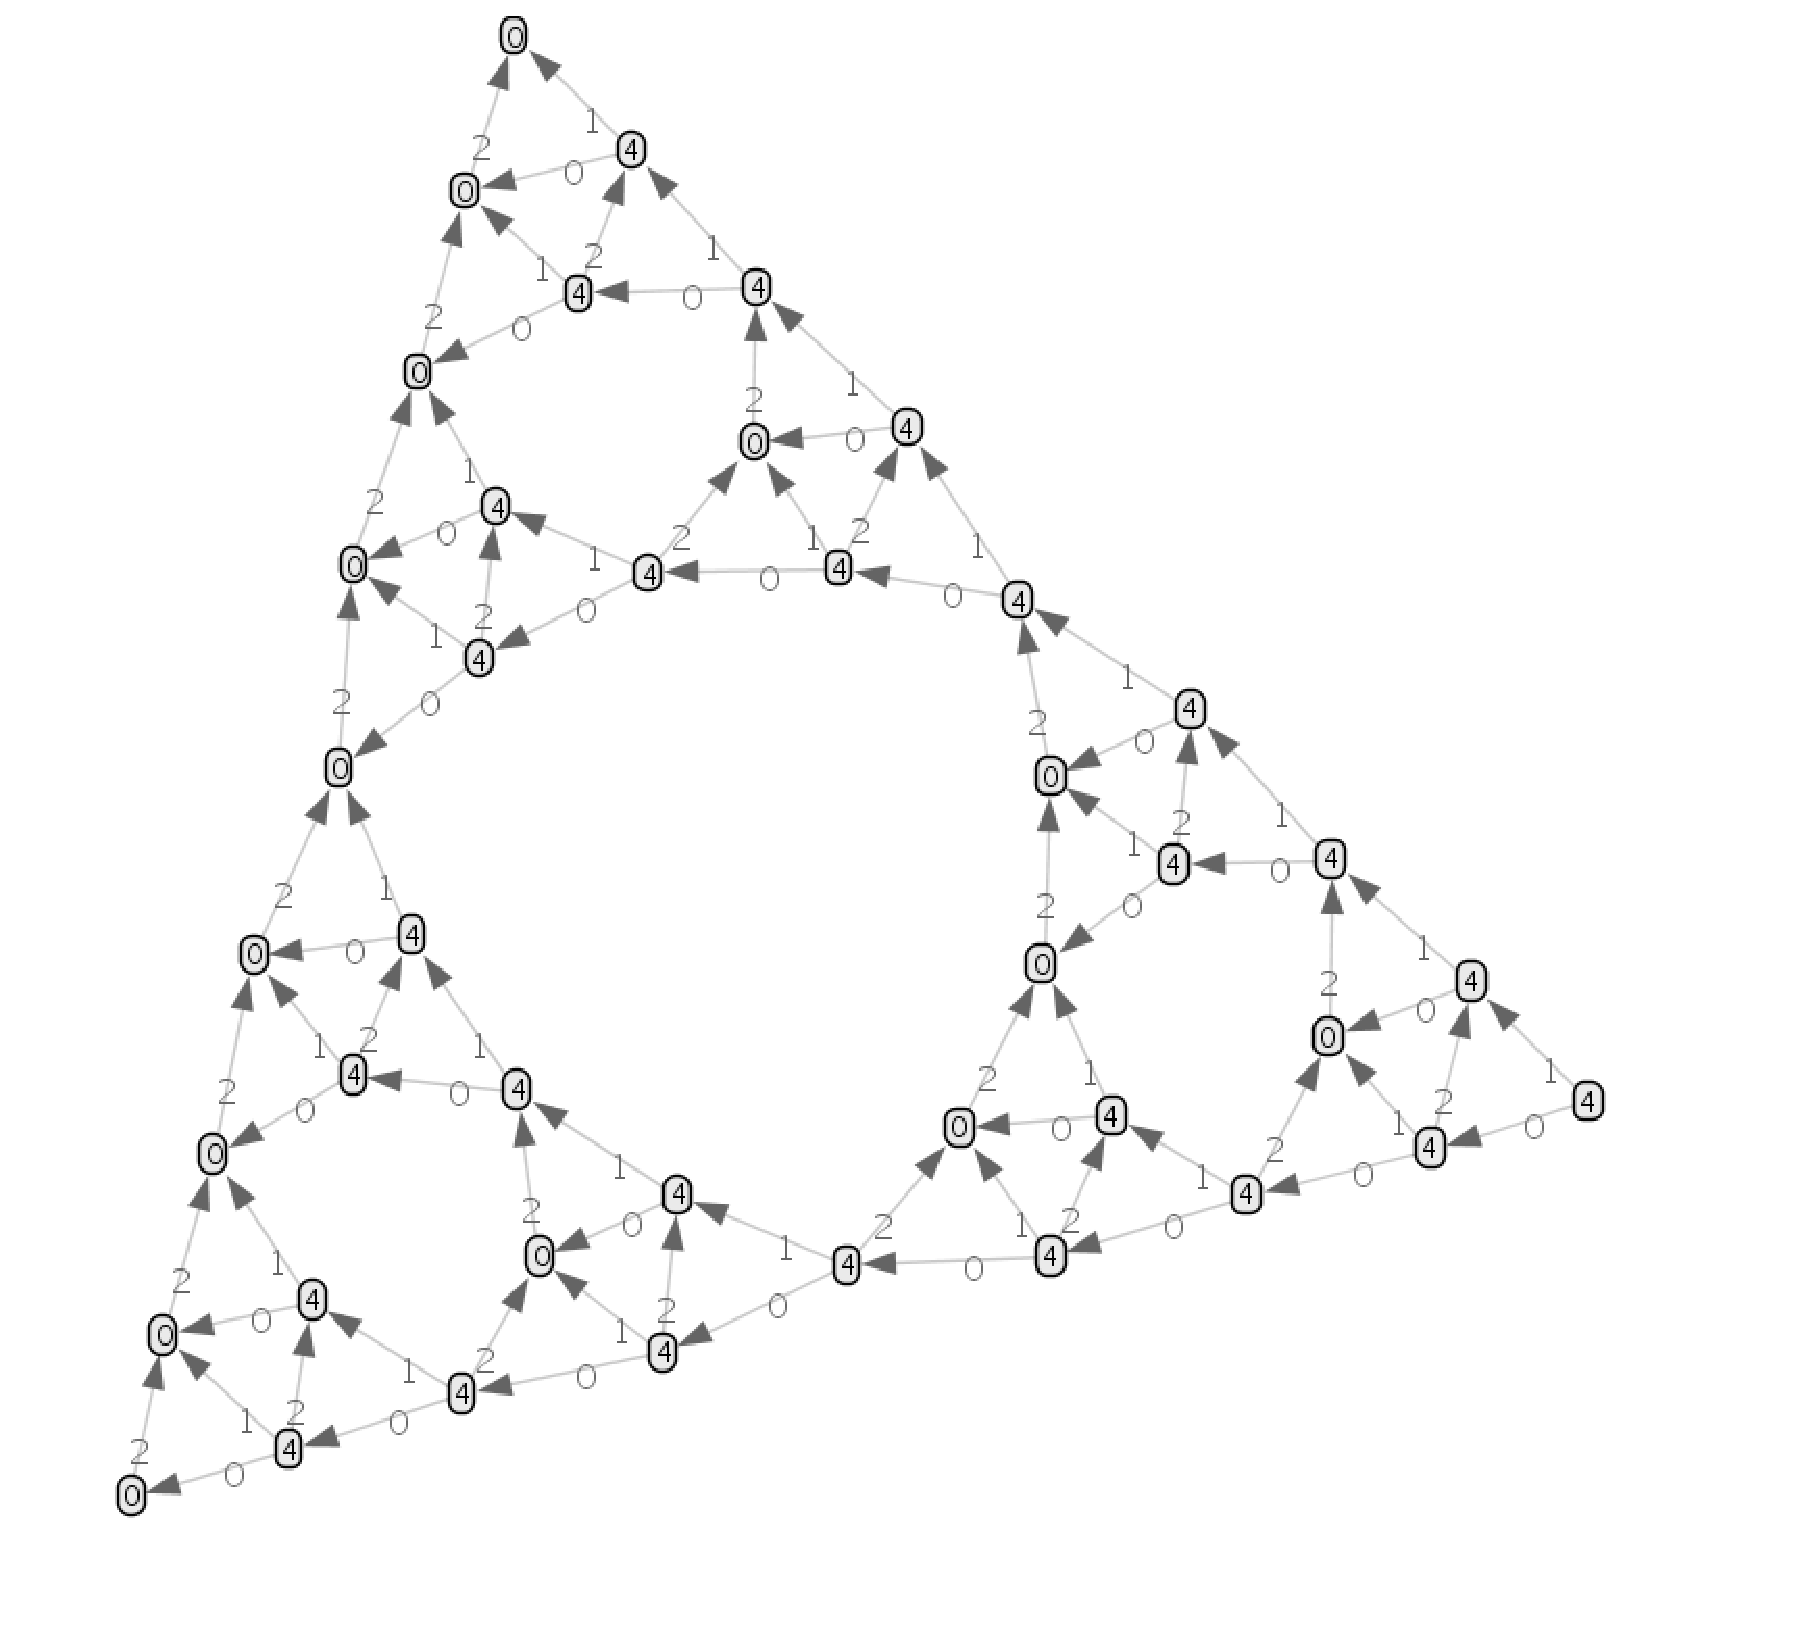
\includegraphics[scale=.4,angle=-15]{sierpinski-3.eps}
 \end{center}
\vspace*{-2.5cm}
\caption{Third generation Sierpinski triangle \label{fig:sierpinski}}
\end{figure}




\section{Implementation}

An flowchart of the reference interpreter is shown in Figure \ref{fig:architecture}. Following that, we present a detailed look at each individual component.

\subsection{Overview}

\begin{figure}
\centering
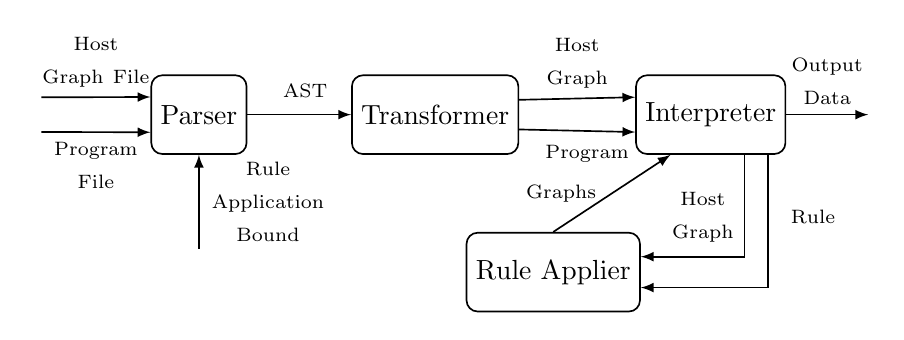
\begin{tikzpicture} [align=center, arrowout]

\node(parser) at (0,0)  [box, rounded corners] {Parser};

\node(gen) at (3,0) [box, rounded corners] {Transformer};

\node(inter) at (6.5,0) [box, rounded corners] {Interpreter};

\node(apply) at (4.5,-2) [box, rounded corners] {Rule Applier};

\draw[arrowout] (-2, 0.22) -- node[above, text width=1.5cm]{\scriptsize{Host Graph File}} (parser.160);
\draw[arrowout] (-2, -0.22) -- node[below, text width=1.5cm]{\scriptsize{Program File}} (parser.200);
\draw[arrowout] (0,-1.7) -- node[right, text width=1.5cm]{\scriptsize{Rule Application Bound}} (parser.270);

\draw [arrowout] (parser) --  (gen);
\node at (1.35,0.3) {\scriptsize{AST}};

\draw [arrowout] (gen.10) -- node[above, text width=1cm]{\scriptsize{Host Graph}} (inter.167);
\draw [arrowout] (gen.350) --  (inter.193);
\node at (4.9,-0.5) [text width=1cm]{\scriptsize{Program}};

\draw [arrowout] (inter.325) |- (apply.350);
\node at (7.8,-1.3) {\scriptsize{Rule}};

\draw [arrowout] (inter.310) |- (apply.10);
\node at (6.4, -1.3) [text width=1cm]{\scriptsize{Host Graph}};

\draw [arrowout] (apply.90) --  (inter.225);
\node at (4.6,-1) {\scriptsize{Graphs}};

\draw[arrowout] (inter) -- node[above, text width=1cm]{\scriptsize{Output Data}} (8.5,0);

\end{tikzpicture}



\caption{Data flow of the reference interpreter.} \label{fig:architecture}
\end{figure}

The interpreter takes three inputs: a file containing the textual representation of a GP2 program, a file containing the textual representation of a host graph, and an upper limit on the number of rule applications to be made before halting program execution. The interpreter runs the program on the host graph until either the bound is reached or the end of the program is reached on all branches. The default output is a complete description of all possible outputs. There is a command-line flag to print only one result in case the total computation is too slow for a particular program.

\subsection{Parser}

We use a parser combinator library fine-tuned to process some syntax specific to GP2. Each nonterminal of the GP2 context-free grammar is a function that parses the right-hand side of its rule. These functions are chained together with combinators. The combinators facilitate the requirements of the parsing step. For example, there is a combinator to parse zero or more of a string, and a combinator to ignore a token with no semantic significance. 

\subsection{Transformation}

The transformation phase extracts some semantic information from the AST, such as the types of variables specified in a rule schema's parameter list, and transforms graphs into an internal representation.

A graph is represented as a pair of extensible arrays: one for the nodes and one for the edges. An array is a list of key-value pairs, where the keys are integers. Node and edge labels are encoded into the node and edge data types. The simplicity of this implementation is intentional. Operations on graphs are concisely represented using Haskell's library of list processing functions. We chose to emphasise simplicity, readability and elegance over performance.

\subsection{The Interpreter}

The interpreter runs the GP2 program on the host graph. In many example programs, the same graph can be reached through several distinct computational branches. Therefore, when program execution is complete, a naive isomorphism checker is used to collate the list of output graphs into its isomorphism classes. The output is as follows:

\begin{itemize}
\item A list of unique output graphs, up to isomorphism, with a count of how many isomorphic copies of each graph were generated.
\item The number of failures. A failure occurs when no rule from a set of rules cannot be applied to a graph, except if the rule set is in a loop or the conditional section of a conditional branching statement.
\item The number of unfinished computations. A computation is unfinished if the bound on rule applications has been reached before the end of the program.
\end{itemize}

During program execution, a list of \texttt{GraphStates} is maintained, representing every possible nondeterministic execution of the program. A \texttt{GraphState} is an abstract data type: its values are a graph along with its rule application count, a failure symbol, and an unfinished symbol. There is a Haskell function to evaluate each GP2 control construct. Each function takes as input a single \texttt{GraphState}, along with some data about the program, and outputs a list of \texttt{GraphStates}. The \texttt{GraphStates} are propagated between functions with the use of recursive calls and Haskell's \texttt{concatMap} function. \texttt{GraphStates} representing failures and unfinished computations remain untouched after their creation, while \texttt{GraphStates} containing an intermediate graph are modified when a rule call is reached in the program's AST. The rule application process is the core of the interpreter, which is discussed in the following sections.


\subsection{Graph Matching}

From a pattern graph $L$ and a host graph $G$, the graph matcher constructs a list of \texttt{GraphMorphisms}. A \texttt{GraphMorphism} is a data structure containing the \textit{environment}, namely the variable-value assignments; a mapping between nodes in $L$ and the corresponding nodes in $G$; and a similar list of edge mappings. Morphisms are generated in two steps. First the node morphisms are constructed, then each node morphism is augmented with appropriate edge mappings if possible. The mappings used are association lists. Like our graph representation, they are simple and easy to manage at the expense of performance.

The node matching algorithm works as follows, where $k$ is the number of nodes in $L$. 

\begin{enumerate}
\item Generate the list of all $k$-sized sets of nodes from $G$.
\item Pair up (with Haskell's \texttt{zip}) each of the above sets with the set of nodes from $L$ to create a list of candidate node morphisms.
\item Remove items from the candidate morphisms list that:
  \begin{itemize}
  \item map a root node to a non-root node.
  \item map a node $l$ to a node $h$ where either the indegree or outdegree of $l$ is greater than that of $h$.
  \item map a node $l$ to a node $h$ where $l$'s mark is not cyan and not equal to $h$'s mark.
  \end{itemize}
\item Iterate through the sets from step 2, comparing the labels of nodes in $L$ to those in $G$. Remove the sets in which node labels do not match for all pairs of nodes. Add any variable-value assignments as necessary.
\end{enumerate}

The three filtering criteria in step 3 are cheap relative to label matching because they perform comparisons on easily-accessible information, in contrast to a full scan of a potentially large GP2 list expression.

It is clear that the complexity of this algorithm increases exponentially with both the size of $L$ and the size of $G$ due to the expensive first step. This is a naive matching strategy that would not be appropriate if performance were a consideration. In this case, where correctness is a greater concern, the simplicity of this algorithm is of benefit by making the source code easier to reason about.


The edge matching algorithm attempts to find an appropriate edge morphism for each node morphism in the list generated above. Valid edge morphisms are added to the data structure and returned as a \texttt{GraphMorphism}. The first step is to generate the list of source-target pairs of each edge in $L$. Then, for each node morphism $NM$:

\begin{enumerate}
\item Translate each source and target pair from $L$ to the pair of their images in $G$, according to $NM$.
\item For each source-target pair in $G$, get the list of edges from the source to the target.
\item Using a zip operation, pair each edge in $L$ with its set of candidate edge matches from the previous step.
\item For each edge in $L$, test its label against the labels of all of its candidate matches. Remove the items in which edge labels do not match. Add any variable-value assignments as necessary.
\end{enumerate}

In this way, the morphisms generated obey the morphism conditions by construction. Furthermore, all morphisms generated are total morphisms. This is because the collection of \textit{all} nodes (edges) in $L$ were tested against candidate node (edge) sets of equal size.


\subsection{Label Matching}

The label matching algorithm establishes whether a label from a rule item can be matched with a label from a host item. It takes as input the current environment and the two labels to be compared. 

GP2 labels consist of a mark and a list. The marks are encoded as an abstract data type and are directly comparable. Lists are naturally represented as Haskell lists, where each element is an atom. Atoms occurring in the host graph are constants (integers, characters or strings), while rule atoms are either constants, variables or a concatenated string. If a variable-value assignment is required to a complete a match, it is tested against the current environment to ensure that the same variable is not mapped to two different values. 

In almost all cases, atoms are directly comparable. The most interesting case occurs if a list variable is encountered. We exploit the fact that only one list variable is allowed in a LHS label (to ensure unique matches). The length of the remainder of the rule list is compared with the length of the remainder of the host list. This information is used either to assign the list variable the list of appropriate length, or to abort matching in the case that there are too few host atoms left to match the remaining rule atoms.

\subsection{Rule Application}

If the graph matcher returned a list of morphisms, each of these morphisms is checked against the dangling condition and any application conditions in the rule itself. Following that, the rule application is performed in the following steps: delete edges, delete nodes, relabel nodes, add nodes, relabel edges, add edges. 

The output of the rule application is a list of graphs, where each graph is the result of a single rule application guided by one of the morphisms returned by the graph matcher.

%In the double-pushout framework of graph transformation, on which GP 2 is based, a rule may not be applicable for a particular match as applying the rule could leave an edge without a source or target. The dangling condition forbids this: it requires that all host edges not deleted by the rule are not incident to nodes deleted by the role.


%\subsection{Rooted graphs}

%Lessons learned from the implementation of the original GP language led to the addition of support for root nodes to GP2. A node carries a simple binary flag indicating whether it is a root node or not. A root node in a rule graph can only match a root node in the host graph, and then only if all other normal matching conditions are met, eliminating a large number of possible subgraph matches with only an inexpensive boolean test. Whereas a non-root node in the rule graph may match a node irrespective of its root-node status.


%Even in the reference interpreter, addition of a root node can result in a significant performance gain.


\section{Performance Evaluation}\label{sec:performanceevaluation}

While not tuned for speed, our reference interpreter still needs to be fast enough to be capable of useful work. In this section we will look at how efficiently it executes the benchmark programs we have described, and what factors affect performance.

% TODO: mention performance of previous versions, and how increased performance brought bugs and limitations to light.


\subsubsection*{Execution environment}

All benchmarking was done on a quad-core Intel i7 clocked at 3.4GHz, with 8GB RAM, running 64-bit Ubuntu 14.04 LTS with kernel 3.13.0.

The GP~2 interpreter is single-threaded, so the number of processor cores should not have a significant impact on the performance.


\subsubsection*{Compilation options}

The interpreter was compiled with GHC version 7.6.3 with optimisations and profiling support enabled, using the following command-line:

\begin{verbatim}
$ ghc -O2 -prof -fprof-auto -rtsopts -o gp2 Main.hs
\end{verbatim}

Profiling information generated by the resulting instrumented binary was used to obtain the numbers presented here, and also to inform the discussion of these results in the next section.


\subsubsection*{Running GP~2}

The \texttt{gp2} executable has three mandatory commandline arguments: a GP~2 program, a host graph on which to run the program, and a upper bound on the number of allowed rule applications.

The rule application bound, $k$ can be used to restrict the size of the search space, only allowing output graphs that can be reached in fewer than $k$ graph transformations. As part of its output, the interpreter reports the number of unfinished computations which halted upon reaching the bound.

% explain commandline options to interpreter (e.g. max apps)

Additionally \texttt{gp2} accepts two optional arguments that control the number of output graphs generated and use of the built-in isomorphism checker:

\begin{description}
	\item[\texttt{--no-iso} \textit{[n]}]  Disable the isomorphism checker. As this can result in a very large number of output graphs, this flag accepts an optional numeric parameter which sets a maximum number of graphs to generate.

	\item[\texttt{--one}] Only produce a single output graph. Equivalent to \texttt{--no-iso 1}.
\end{description}

Benchmarks were run using the following commandline. We limited execution time to 5 minutes per program/host graph pair. The rule application bound was set sufficiently high that the limit is not reached in any of the benchmarks being run.

\begin{verbatim}
$ timeout --foreground 5m time \
      gp2 +RTS -p -sgc.prof -RTS $GPOPT $PROG $GRAPH 1000000
\end{verbatim}

Each benchmark was run twice: once with \texttt{\$GPOPT} set to \texttt{--one} (single-output graph mode) and once with it unset (all possible results mode).

An unfortunate property of the Haskell memory profiler is that memory profiling information is not saved to disk if the running program is killed by an external process such as the \texttt{timeout} command, which means we are unable to give accurate figures for memory usage for benchmarks which did not complete within the allotted time.


\subsection{Host Graphs}
\label{subsec:hosts}

Host graphs used for benchmarking are named to give an indication of their overall structure.


\paragraph*{Linear $n$}

A chain of $n$ nodes. The first node has only a single outgoing edge. The last node has only a single incoming edge, and all other nodes have exactly one incoming and one outgoing edge.

\paragraph*{Cyclic $n$}

As Linear $n$, but with an extra edge linking the first and final placed nodes so that every node has exactly one incoming and one outgoing edge.

\paragraph*{$x \times y$ Grid}

A square lattice of $x$ nodes wide by $y$ nodes tall.

\paragraph*{Gen $n$}

The Sierpinski program expects a host graph containing a single node with a numeric label, which is used as the number of iterations of the \texttt{expand!} rule to run.


The \textit{shortest distances} benchmark requires additional information in the form of costs for traversing each edge. For all of the host graphs for this program, half of the edges were assigned a cost of one and half were assigned a cost of two.




\begin{table}[h]
\begin{minipage}{\textwidth}
\centering

\begin{tabular}{llrrcrr}
\hline 
&  & & & & \multicolumn{2}{c}{Heap/kB}\\
Benchmark          & Host Graph\footnotemark & Apps & Time/s   & & Allocd & Live \\
\hline 
Acyclicity test
 &             3x3 grid &    12 &    0.02 & &  2048 &   129 \\
 &             5x5 grid &    40 &    0.03 & &  3072 &   382 \\
 &             7x7 grid &    84 &    0.17 & &  4096 &  1119 \\
 &             9x9 grid &   144 &    0.70 & &  6144 &  2100 \\
 &           cyclic 100 &     0 &    0.04 & &  3072 &   778 \\
 &           cyclic 500 &     0 &    0.46 & & 14336 &  5646 \\
 &          cyclic 1000 &     0 &    1.76 & & 25600 & 10368 \\
\hline
Shortest distances
 &             5x5 grid &    38 & $<0.01$ & &  3072 &   414 \\
 &             7x7 grid &    90 &    0.08 & &  4096 &  1177 \\
 &             9x9 grid &   175 &    0.39 & &  8192 &  3172 \\
\hline
Sierpinski
 &                gen 2 &     7 & $<0.01$ & &  2048 &   133 \\
 &                gen 3 &    17 &    0.14 & &  5120 &  1056 \\
 &                gen 4 &    45 &    6.52 & & 58368 & 18313 \\
 &                gen 5 & - & $>5m$ & & - & - \\
\hline
Transitive closure
 &            linear 05 &     6 & $<0.01$ & &  2048 &   144 \\
 &            linear 10 &    36 &    0.04 & &  2048 &   144 \\
 &            linear 20 &   171 &    1.67 & & 21504 &  7073 \\
 &            linear 30 &   406 &   14.39 & & 103424 & 33152 \\
 &            linear 40 &   741 &   66.31 & & 324608 & 103275 \\
 &            linear 50 & - & $>5m$ & & - & - \\
\hline
Vertex colouring
 &             3x3 grid &    27 &    0.02 & &  2048 &   140 \\
 &             5x5 grid &   125 &    0.03 & &  3072 &   999 \\
 &             7x7 grid &   343 &    0.17 & &  9216 &  3681 \\
 &             9x9 grid &   729 &    0.89 & & 25600 & 11438 \\
\hline

\end{tabular}

\caption[Reference interpreter benchmarks]{Reference interpreter benchmark results when generating a single output graph}

\label{table:resultsSingle}
\end{minipage}
\end{table}



\begin{table}[h]
\begin{minipage}{\textwidth}
\centering

\begin{tabular}{llrrrrrcrr}
\hline 
&  & \multicolumn{3}{c}{Output Graphs} & & && \multicolumn{2}{c}{Heap/kB}\\
Benchmark          & Host Graph\footnotemark & Total & Unique   & Failed & Apps & Time/s   & & Total  & Live \\
\hline 
Acyclicity test
 &             2x2 grid &      6 &         1 &     0 &     4 & $<0.01$ & &  2048 &   134 \\
 &             3x3 grid &  19770 &         1 &     0 &    12 &   12.00 & & 10240 &  3301 \\
 &             4x4 grid & - & - & - & - & $>5m$ & & - & - \\
 &           cyclic 100 &      0 &         0 &   100 &     0 &    0.06 & &  4096 &   784 \\
 &           cyclic 500 &      0 &         0 &   500 &     0 &    0.86 & & 14336 &  5651 \\
 &          cyclic 1000 &      0 &         0 &  1000 &     0 &    3.31 & & 26624 & 11053 \\
\hline
Shortest distances
 &             2x2 grid &      6 &         1 &     0 &     4 & $<0.01$ & &  2048 &   131 \\
 &             3x3 grid &  28924 &         1 &     0 &  9-14 &   19.15 & & 167936 & 58180 \\
 &             4x4 grid & - & - & - & - & $>5m$ & & - & - \\
\hline
Sierpinski
 &                gen 2 &      6 &         1 &     0 &     7 &    0.04 & &  3072 &   242 \\
 &                gen 3 & - & - & - & - & $>5m$ & & - & - \\
\hline
Transitive closure
 &            linear 05 &    866 &         1 &     0 &     6 &    0.44 & &  6144 &  1699 \\
 &            linear 10 & - & - & - & - & $>5m$ & & - & - \\
\hline
Vertex colouring
 &             2x2 grid &    480 &         2 &     0 &   6-8 &    0.07 & &  5120 &  1598 \\
 &             3x3 grid & - & - & - & - & $>5m$ & & - & - \\
\hline

\end{tabular}

\caption[Reference interpreter benchmarks]{Reference interpreter benchmark results when generating all possible output graphs}

\label{table:resultsAll}
\end{minipage}
\end{table}


\subsection{Benchmark performance}

Tables \ref{table:resultsSingle} and \ref{table:resultsAll} summarise the reference interpreter performance for the five benchmark programs, each run on several host graphs. Table \ref{table:resultsAll} shows figures for generating all possible results for each program/host-graph pair, while table \ref{table:resultsSingle} shows results when the interpreter is running in single output graph mode.



Comparing tables \ref{table:resultsAll} and \ref{table:resultsSingle} gives an indication of the additional costs associated with generating all graphs and isomorphism-checking the results.



% Generating all possible intermediate graphs

\subsubsection*{Exhaustive search}

When viewing the results in \ref{table:resultsAll}, it should be remembered that the interpreter is computing \textit{all possible} output graphs for a given program/host-graph pair, then consolidating the results based on isomorphism. It is therefore unsurprising that execution time increases exponentially with increasing size of host graph.

However, as already mentioned, more consideration was given to code-correctness and readability than to execution speed or memory consumption.

While performance is acceptable for some quite complex programs, it is nevertheless easy to find cases in which performance rapidly degrades to an unacceptable degree. A particular example being the vertex-colouring benchmark program, which exhibits exponential growth in the number of possible intermediate graphs with increasing edge counts.

One of the most serious limits on the performance of the reference interpreter, which impacts matching of any non-trivial rule, is the naive node-matching strategy. Given a rule with $n$ nodes, select all permutations of $n$ nodes from the host graph, then discard those that fail to meet rootedness, label and edge constraints.

While from the point of view of simplicity this is a reasonable choice for finding all possible outputs for each rule, it is far from an optimal way of finding a single output graph; for any non-trivial rule and host pair the chances of $n$ nodes selected essentially at random matching a rule is very low, meaning that many permutations need to be inspected for each successful match.

That this strategy is repeated for all of the intermediate graphs generated by the previous rule application explains the combinatorial explosions we see in heavily non-deterministic programs like \textit{Sierpinski} and \textit{Shortest distances}.

% interpreter cost vs compiler
\subsubsection*{Interpreter costs}

Any interpreter has run-time costs which would be paid at compile-time in a compiler. These costs can account for a significant percentage of the execution time.

In the sub-second execution time benchmarks, profiling information indicated that a significant portion of the execution time was spent parsing the rule-graphs and building map structures.


\subsubsection*{Separate graph and edge matching}

As discussed in section \ref{sec:graph-match} the reference interpreter matches nodes and edges in separate passes. This makes for a simple algorithm at the expense of performance.

A more performance focussed implementation would use a \textit{search plan}\cite{Horvath-Varro07} in which a graph morphism is built incrementally by adding nodes and edges to an existing partial morphism, and back-tracking if no suitable graph elements could be found.


\subsubsection*{Generic data structures}

The current version of the interpreter uses a generic lazy map data structure which gives a reasonable balance between cost of search and cost of update. 


Our first prototypes stored the graphs as linked-lists of key/value pairs. The result was an interpreter which spent most of its execution time traversing these lists retrieving nodes and edges. Switching to the faster map structure alone yielded a factor of two speed improvement.

Nevertheless, an underlying data structure tuned to our specific usage patterns and judiciously indexed could dramatically reduce this high cost of node and edge retrieval.


\subsubsection*{Isomorphism checking}

Another cost associated with generating all possible output graphs is isomorphism checking. In benchmarks where nondeterminism gives us multiple ways of reaching similar output graphs we want a way of reducing this potentially large set of outputs to those which are truly distinct. A particularly extreme example of this can be seen in the \textit{3x3 grid} host graph of the \textit{Shortest distances} benchmark. Here we produced nearly 30~000 isomorphic output graphs! Presumably if allowed to run to completion the \textit{4x4 grid} would yield several orders of magnitude more.


% Cost of profiling
\subsubsection*{Profiling costs}

We have also incurred some incidental costs by gathering the profiling information used to generate 

% TODO: guestimate profiling costs


% TODO: fail early and fail cheaply!

\section{Related and Future Work}
\label{sec:relatedandfuture}
Early programming languages were often defined by their implementations,
perhaps in the form of a \emph{definitional interpreter}.
Despite the development of more abstract techniques
for defining the operational semantics of programming languages, in recent years there
have been several efforts to rehabilitate definitional or
reference interpreters, sometimes informed by more abstract semantic
presentation.
Motivation varies, but here are representative remarks in the preface
of an influential textbook: 
\begin{quote}
\textit{Our goal is to provide a deep, working understanding of the essential concepts of programming languages. \ldots
Most of these essentials relate to the semantics, or meaning, of program elements. Such meanings reflect how program elements are interpreted as the program executes. Programs called interpreters provide the most direct, executable expression of program semantics. \ldots We therefore choose interpreters as our primary vehicle for expressing the semantics of programming language elements. \ldots
The most interesting question about a program as object is, \textnormal{``What does it do?''} The study of interpreters tells us this. Interpreters are critical because they reveal nuances of meaning, and are the direct path to more efficient compilation and to other kinds of program analyses.} \cite{Friedmanetal2008}
\end{quote}
In several respects, our motivation is similar.  We aim to promote a ``\textit{deep, working understanding}'' of the GP2 design, and to find ``\textit{path(s) to more efficent compilation \ldots and program analysis}''.

Languages based on graph-transformation rules include
%Fujaba?
\textsc{Progres} \cite{Schuerr-Winter-Zuendorf99a},
\textsc{Agg} \cite{Ermel-Rudolf-Taentzer99a,Runge-Ermel-Taentzer11a},
\textsc{Gamma} \cite{Fradet-LeMetayer98a},
\textsc{Groove} \cite{Ghamarianetal12},
\textsc{GrGen.Net} \cite{JakumeitBuchwaldKroll2010} and
\textsc{Porgy} \cite{Fernandez-Kirchner-Mackie-Pinaud14a}.
To our knowledge, none of these languages has a published implementation in the same spirit as our reference interpreter. For example, \textsc{Groove} and \textsc{GrGen.Net} are two of the most widely used systems. The Java source code for the \textsc{Groove} implementation, including a graphical development suite, extends to around 150,000 lines. \textsc{GrGen.Net} is implemented in a combination of Java and C\#: a Java front-end is used to generate C\# code and .NET assemblies from a textual specification of a \textsc{GrGen} program; the run-time system and other components are written in C\#. In all there are around 68,000 lines of Java source for the front-end, and around 93,000 lines of C\# for the run-time system, API support and an interactive shell.
We recognise that both \textsc{Groove} and \textsc{GrGen.Net} are mature and fully-featured systems, and \textsc{GrGen.Net} in particular is highly optimising. Even so, the contrast with the 1000-line Haskell sources for our GP 2 reference interpreter is striking.

\section{Conclusions}
\label{sec:conclusions}

%\subsection{Contributions}

%This work lays a valuable foundation for checking the correctness of subsequent GP2 interpreters and compilers. It also demonstrates the use of a lazy functional language to implement a nondeterministic language. Perhaps the data from running the interpreter on our test programs may reveal some insights into properties/features of the interpreter.






\bibliography{bibliography}{}
\bibliographystyle{plain}
\end{document}
